\documentclass[12pt]{article}

\usepackage{amsmath}
\usepackage{graphicx}
\usepackage{hyperref}
\usepackage[margin=1.2in]{geometry}

\providecommand{\eqn}[1]{eqn.~(\ref{eqn:#1})}
\providecommand{\tab}[1]{Table~\ref{tab:#1}}
\providecommand{\fig}[1]{Figure~\ref{fig:#1}}

\providecommand{\vecsymbol}[1]{\ensuremath{\boldsymbol{#1}}}
\providecommand{\pv}{\vecsymbol{p}}
\providecommand{\deltav}{\vecsymbol{\delta}}

\title{Tech Note on Quality Assurance for DESI Spectroscopic Reduction \\
\vspace{5mm}{\large\bf DESI-doc-XXX-v1}}
\author{J. Xavier Prochaska, others}

\begin{document}
\maketitle

\section{Introduction}

This technical note summarizes the Quality Assurance outputs for the
{\tt desispec} package, including both the full spectroscopic pipeline
and the Quicklook pipeline (run on mountain).

This document is maintained in the {\tt desispec} package\footnote{Maintained in the public github repository at \url{https://github.com/desihub/desispec}} under {\tt doc/tex/}
and also summarizes on the DESI Wiki at 
\url{https://desi.lbl.gov/trac/wiki/Pipeline/QualityAssurance}. 

\section{General Architecture}

The QA analysis is performed within the scripts for each
of the primary spectroscopic pipeline steps (e.g.\ fiberflat,
sky subtraction, fluxing).   The QA code is located within 
the individual modules and called from within the individual
scripts.  A basic framework for controlling and packaging
QA analysis is provided in {\tt qa\_exposure.py}
within the {\tt desispec/py/qa} folder.
All plotting codes will be kept within the module
{\tt qa\_plots.py} in the same folder.

QA metrics are stored
in a YAML file, one per exposure/camera/tile to allow for
multi-processing.  Likewise, QA figures are stored in a 
PDF file per exposure/camera/tile combination.
The naming convention for these files is 
{\tt qa}-{\tt camera tile}-{\tt exposure}.yaml or
{\tt qa}-{\tt camera tile}-{\tt exposure}.pdf, 
e.g. {\tt qa-b0-00000002.pdf}.

For compactness, it is likely that these files will be collated
once the processing of all tiles of a given exposure is complete.
This is not yet implemented.

\section{PSF}

\section{Flat Fielding}

\subsection{Overview}

The primary goals of QA for flat fielding are:

\begin{itemize}
\item Crudely assess system throughput (i.e.\ sufficient counts)
\item Assess flat field model
\item Identify bad fibers
\item Assess flat field within and across tiles
\item Assess flat field versus time
\end{itemize}

\subsection{Metrics}

The QA analysis for the fiberflat step is guided by a set of 
parameters defined in {\tt qa\_exposure.QA\_Frame.init\_fiberflat}.
In the case of fiberflat analysis, these parameters are used 
to raise warnings if the QA metrics exceed these pre-defined values.
Table~\ref{tabl:flat_param} summarizes the parameters.

\begin{table}[h]
\begin{center}
\caption{Fiberflat QA Parameters}
\label{tab:flat_param}
\begin{tabular}{lcl}
\hline
{\bf Name} & {\bf Value} & {\bf Brief Description}\\
\hline
MAX\_N\_MASK    & 20000 & Maximum number of pixels masked in fit \\
MAX\_SCALE\_OFF & 0.05  & Maximum fractional offset between model and individual fibers \\ 
\hline
\end{tabular}
\end{center}
\end{table}


Table~\ref{tab:flat_metrics} summarizes the QA metrics measured
for the fiberflat step.  

\begin{table}[h]
\begin{center}
\caption{Fiberflat QA Metrics}
\label{tab:flat_metrics}
\begin{tabular}{ll}
\hline
{\bf Name} & {\bf Brief Description}\\
\hline
N\_MASK    & Number of pixels masked in fit for all fibers \\
\hline
\end{tabular}
\end{center}
\end{table}


Here is an summary of each:



\noindent
{\tt N\_MASK}:  This metric records the number of pixels that were
masked during the fiberflat fit.  It is the total over all fibers.


\subsection{Plots}

%%%%%%%%%%%%%%%%
\section{Sky Subtraction}

The primary goals of QA for sky subtraction are:

\begin{itemize}
\item Assess residuals (global)
\item Assess residuals (on sky lines)
\item Assess outliers
\item Examine performance within and across tiles
\item Examine performance vs.\ time
\end{itemize}

%\begin{figure}[htb]
%\begin{center}
%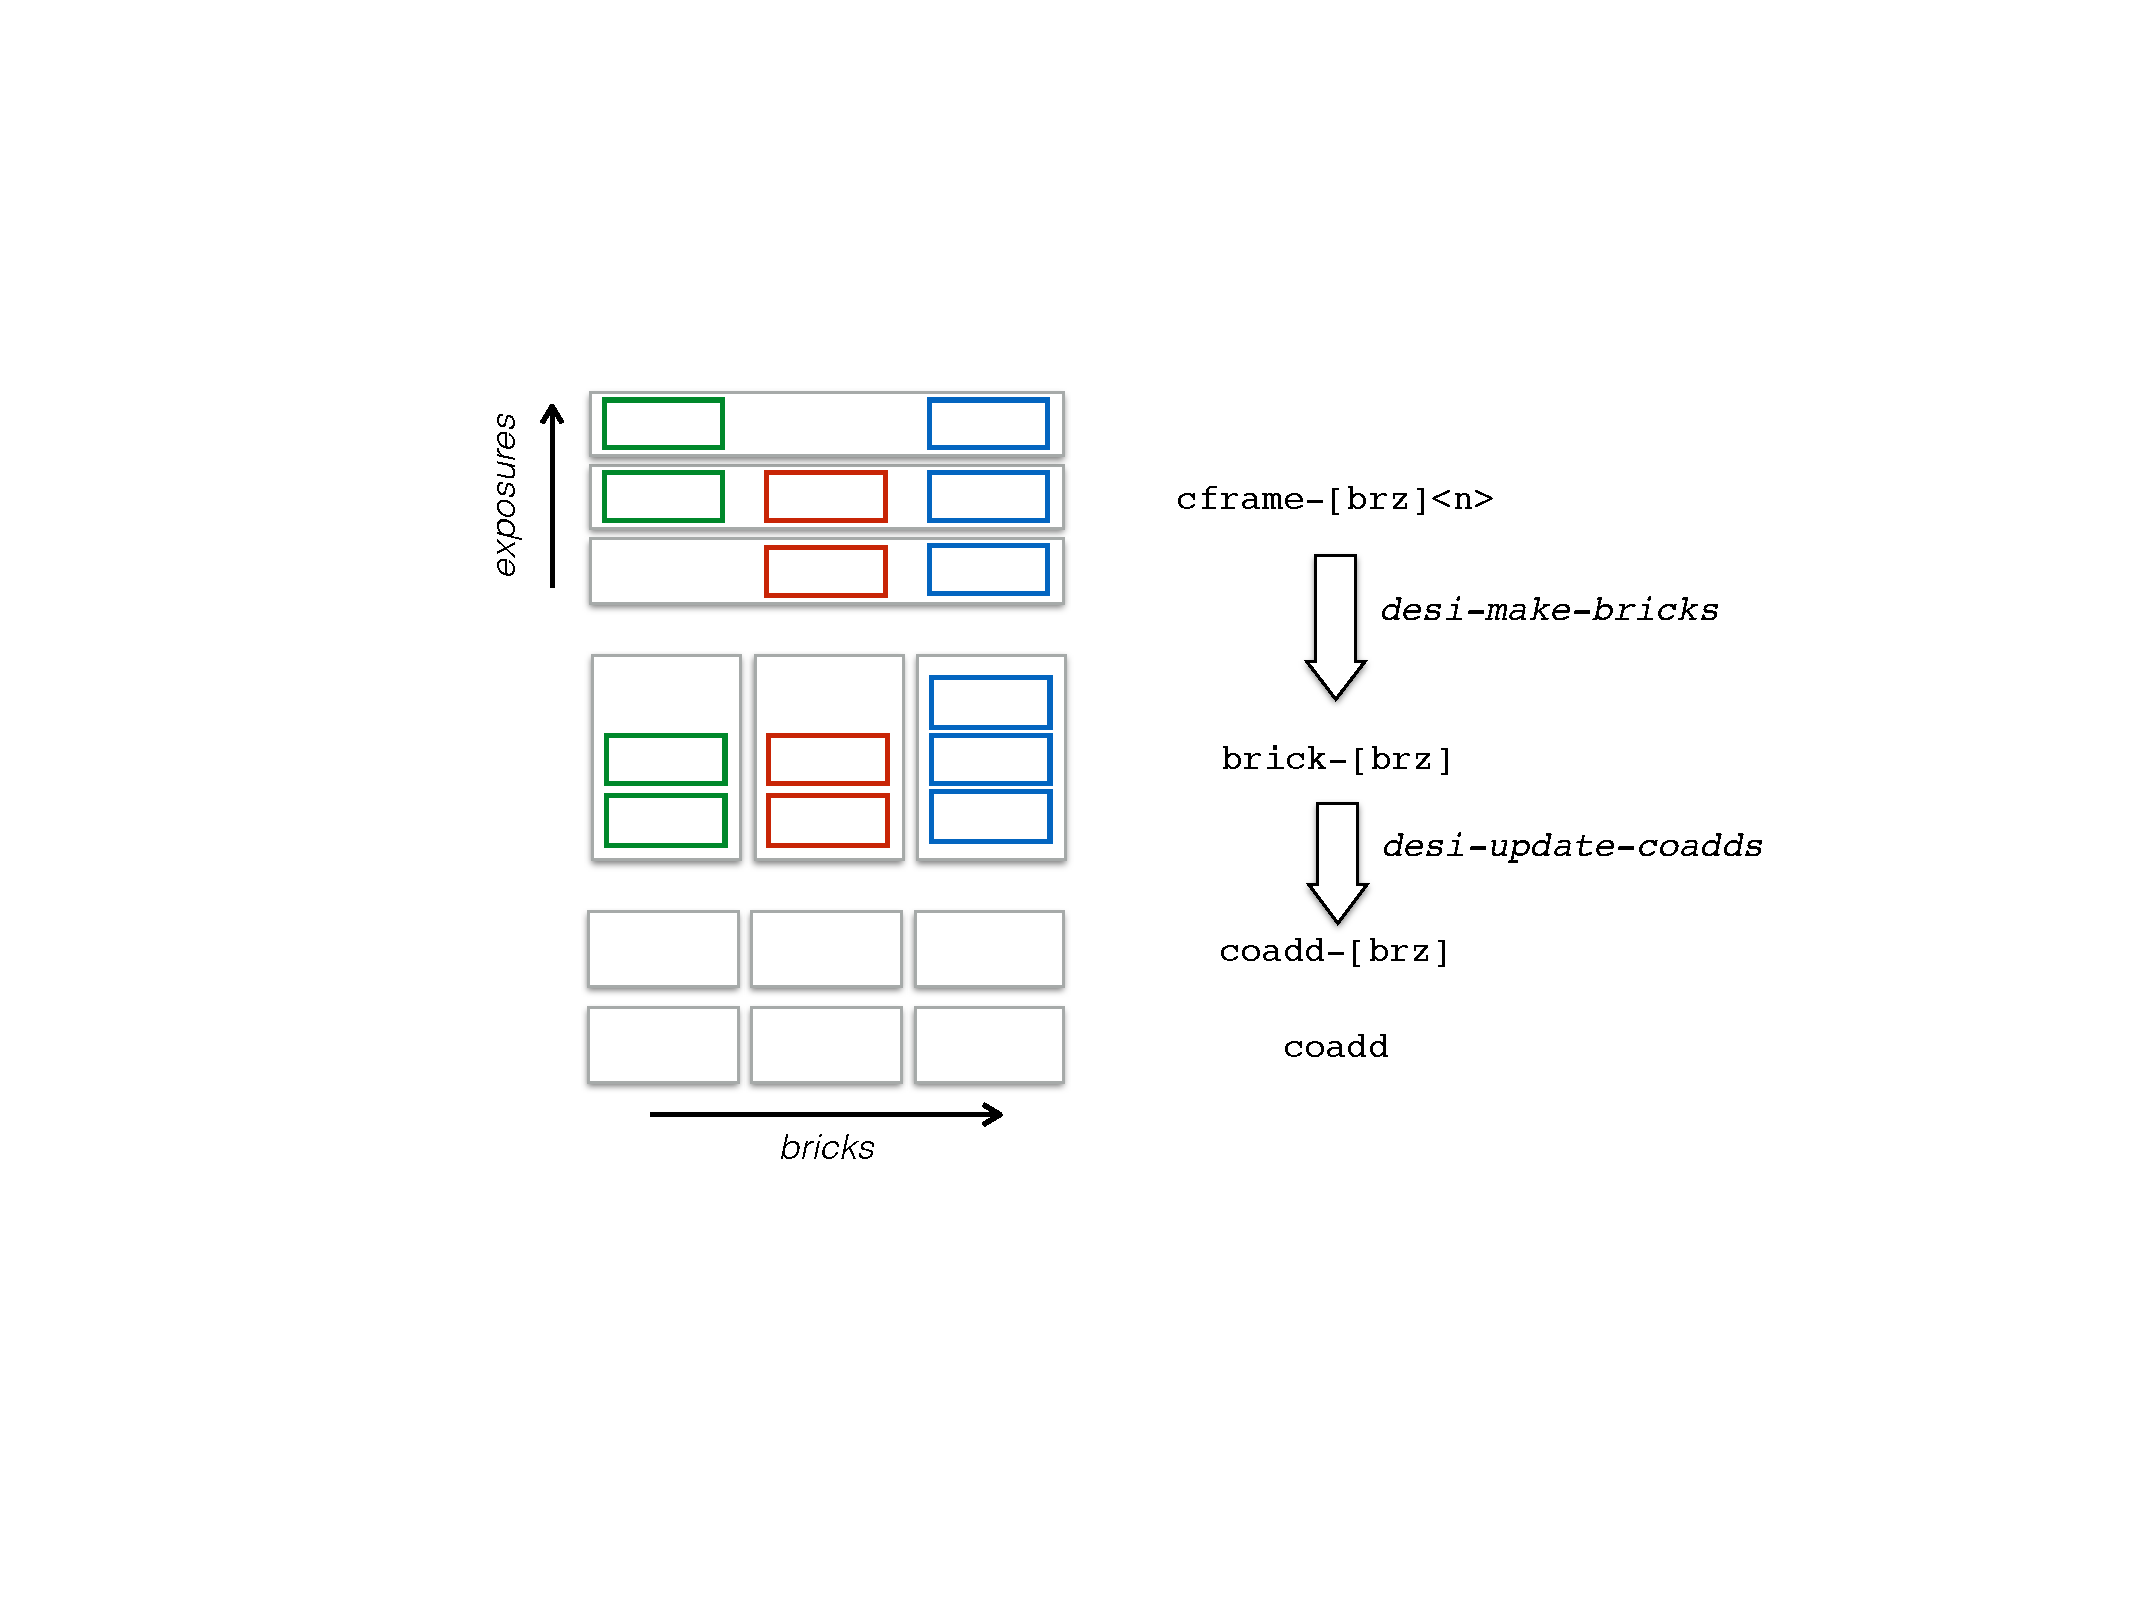
\includegraphics[width=5in]{fig/dataflow}
%\caption{Schematic representation of the coaddition dataflow. Nightly exposures are reduced to cframes (horizontal gray boxes) each covering multiple bricks (colored boxes). The {\tt desi-make-bricks} program repackages the cframe spectra into brick files (vertical gray boxes) containing all of the spectra observed for targets within a single brick. Finally, the {\tt desi-update-coadds} program reads spectra from a single brick file and generates the per-band and global coadd files (gray boxes at the bottom of the diagram).}
%\label{fig:dataflow}
%\end{center}
%\end{figure}


\def\apjl{ApJL} %Astrophysical Journal Letters
\def\aj{AJ} %Astronomical Journal
\def\apj{ApJ} %Astrophysical Journal
\def\pasp{PASP} %Publications of the Astronomical Society of the Pacific
\def\spie{SPIE} %
\def\apjs{ApJS} %Astrophysical Journal Supplement
\def\araa{ARAA} %Annual Review of Astronomy and Astrophysics
\def\aap{A\&A} %Astronomy and Astrophysics
\def\aaps{A\&A~Supl.} %Astronomy and Astrophysics Supplement
\def\nat{Nature} %Nature
\def\nar{New Astron. Rev.} %New Astronomy Review
\def\mnras{MNRAS} %Monthly Notices of the Royal Astronomical Society
\def\jcap{JCAP} %Journal of Cosmology and Astroparticle physics
\def\prd{{Phys.~Rev.~D}}        % Physical Review D
\def\physrep{{Phys.~Reports}} % Physics Reports

\bibliographystyle{plain}
\bibliography{coadd}

\end{document}
